\documentclass[oneside,a4paper,spanish,links]{amca}
%
\usepackage{graphicx}
\usepackage{amsmath,amsfonts}
\usepackage[utf8]{inputenc}
%
\title{PREPARACIÓN Y SIMULACIÓN DE CASO 3D EN OPENFOAM}
%
\englishtitle{SETUP AND SIMULATION OF 3D CASE IN OPENFOAM}

\author[a]{Guillermo Rolle}
%\author[b]{Segundo B. Autor}
%\author[b]{Tercer C. Autor}
%\author[a]{Cuarto D. Autor}
%
%\affil[a]{Grupo de Mecánica Computacional, Universidad Nacional de
%Villa Carolina, Los Alerces 3492, 4200~Villa Carolina, Argentina,
%gmc@uncarolina.edu.ar, \url{http://www.uncarolina.edu.ar/gmc}}
%
%\affil[b]{Grupo de Ingeniería Aplicada, Universidad Nacional de La
%Meseta, Los Cipreses 3493, 4201~La Meseta, Argentina,
%gia@unmeseta.edu.ar, \url{http://www.unmeseta.edu.ar/gia}}

%% NOTA: SI TODOS LOS AUTORES TIENEN LA MISMA AFILICACION
%% USE EL MACRO `\voidaffil' PARA EL CODIGO DE AFILICACION.
%% Ejemplo:
%% \author[\voidaffil]{Primer A. Autor}
%% \author[\voidaffil]{Segundo B. Autor}
%% \author[\voidaffil]{Tercer C. Autor}
%% \author[\voidaffil]{Cuarto D. Autor}
%% %
%% \affil[\voidaffil]{Grupo de Mecánica Computacional,
%% Universidad Nacional de Villa Carolina,
%% Los Alerces 3492, 4200 Villa Carolina, Argentina,
%% gmc@uncarolina.edu.ar, http://www.uncarolina.edu.ar/gmc}

\begin{document}
\vspace{3cm}

\maketitle

%% To set PDF METADATA: uncomment and replace fields in
%% UPPERCASE with appropriate values.
%%
%% \hypersetup{
%%   pdfauthor={AUTHORS},
%%   pdfkeywords={KEYWORDS},
%%   pdftitle={TITLE}
%% }
%%
%% For instance
%% \hypersetup{
%%   pdfauthor={Sponge B. and Star P.},
%%   pdfkeywords={multiphase flow, air-liquid mixtures},
%%   pdftitle={A new model for multi-phase flow}
%% }
%%
%% NOTE: To set the metadata is recommended but not absolutely
%% neccesary.
%% This was done before with the \pdfinfo command,
%% but according to this post:
%% http://de.nntp2http.com/comp/text/tex/2008/12/5358fd061de9703a781885a5dcf98364.html
%% if `hyperref' is used, then you must use \hypersetup{} not \pdfinfo{}

\begin{keywords}
CFD, OpenFOAM, FreeCAD, simpleFoam, scalarTransportFoam
\end{keywords}

\begin{abstract}
Este documento provee información e instrucciones para realizar una simulación de un caso 3D en OpenFOAM.
La geometría 3D se modela con software FreeCAD y se malla con snappyHexMesh. Luego, se ejecutan las simulaciones correspondientes con simpleFoam y scalarTransportFoam.  Se mantienen las condiciones de contorno e iniciales de los informes anteriores. El documento finaliza con conclusiones sobre el caso y los resultados obtenidos. \\
%
\linebreak
%
\textbf{Keywords:} CFD, OpenFOAM, FreeCAD, simpleFoam, scalarTransportFoam\\
%
\linebreak
%
\textbf{Abstract.} This document provides information and
instructions to setup a 3D OpenFOAM case. The geometry is defined with FreeCAD software and is meshed with snappyHexMesh. Afterwards, the corresponding simulations will be run using solvers simpleFoam and scalarTransportFoam. Initial conditions and boundary conditions are kept from previous reports. The document ends with conclusions about the case and the results obtained.
%\\
%\\
%\textbf{Agradecimientos:} Los autores agradecen... (no más de 2 líneas)
% LOS AGRADECIMIENTOS EN LA PRIMERA PAGINA SE PERMITEN SOLO PARA
% PRESENTACIONES DE RESUMENES (NO PARA ARTICULOS COMPLETOS)
\end{abstract}

\section{INTRODUCCIÓN}
En este documento se detallan los pasos a seguir para preparar y ejecutar una simulación en 3 dimensiones con OpenFOAM (ver figura \ref{fg:intro}). Se modela la geometría con software FreeCAD. El caso descrito en este informe se puede descargar del repositorio público: \url{https://github.com/guillerolle/casos_cfd/tree/master/03}. En el repositorio se encuentran también los archivos para FreeCAD.

Se asume que el lector tiene una versión de FreeCAD disponible y lista para utilizar en conjunto con OpenFOAM. No se hará demasiado hincapié en el modelado de la geometría, sino más bien en todo lo que implique a OpenFOAM y CFD en sí.

\begin{figure*}[htb]
	\centerline{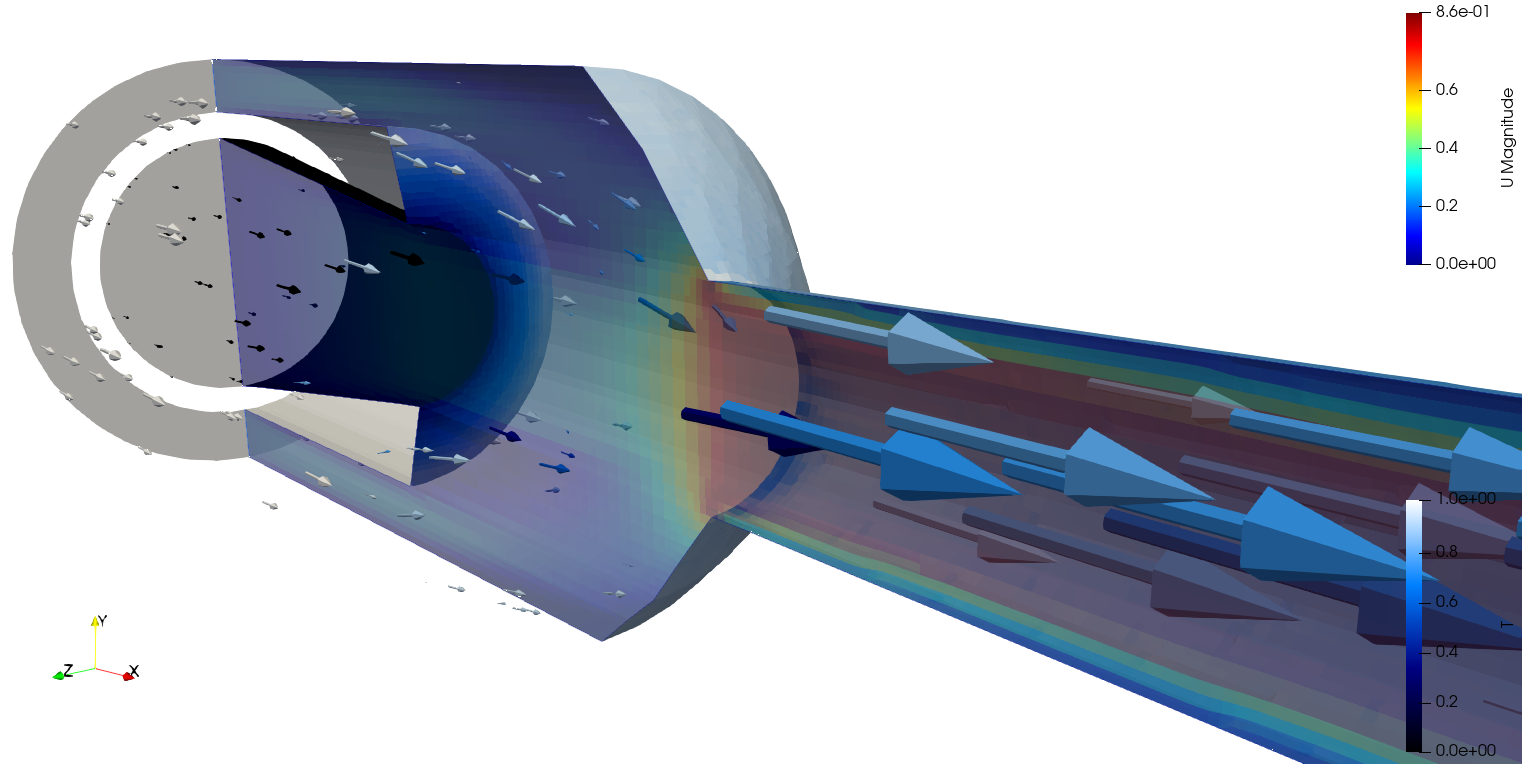
\includegraphics[width=0.8\textwidth]{Figuras/05_GLYPH.png}} \caption{Caso 3D en cuestión} \label{fg:intro}
\end{figure*}

Este informe es parte de la serie de informes de \url{https://github.com/guillerolle/informes_cfd}. Estos casos están basados en un mezclador de agroquímicos en línea.

\section{PREPARACIÓN DE LA GEOMETRÍA}
El primer paso es realizar el modelo en FreeCAD del espacio de fluido que usaremos en la simulación. Es decir, nuestro volumen de control (macroscópicamente). En la figura \ref{fg:boceto_revo} se muestra el boceto del modelo. 

\begin{figure*}[htb]
	\centerline{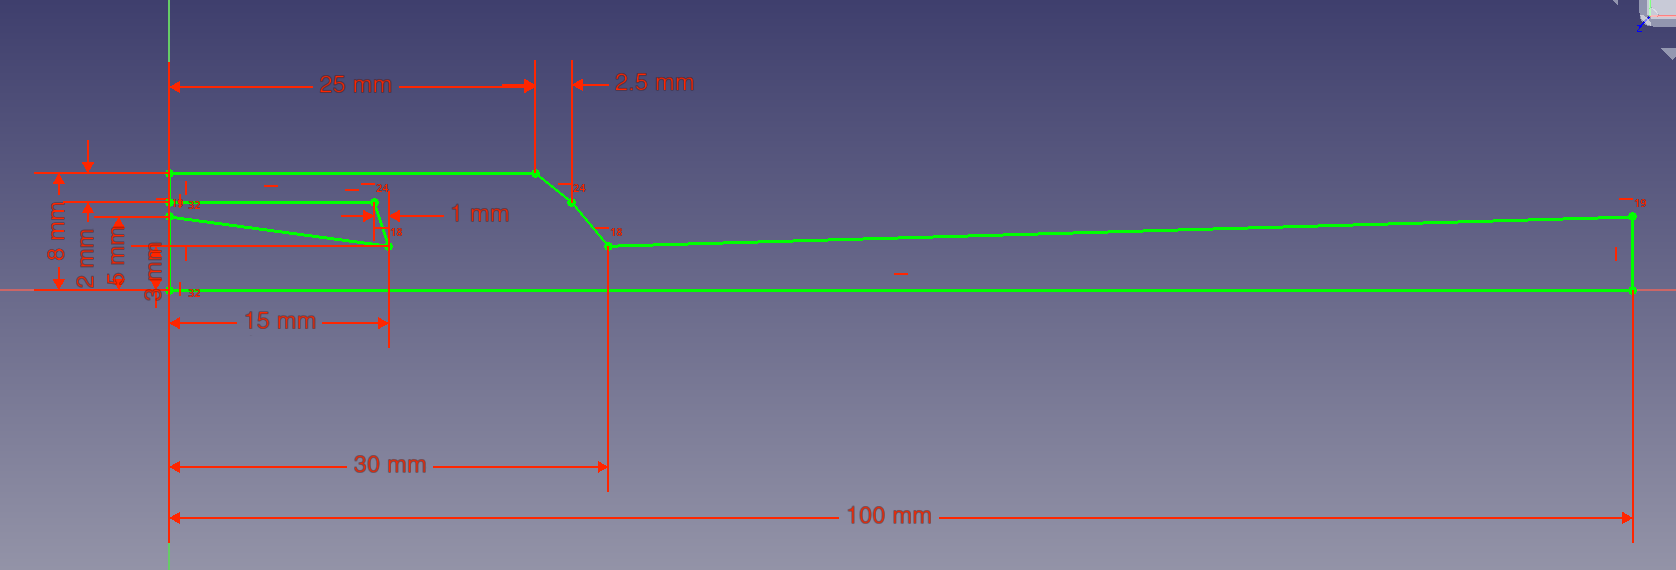
\includegraphics[width=0.8\textwidth]{Figuras/02_BOCETO_REVOLUCION.png}} \caption{Croquis de la geometría} \label{fg:boceto_revo}
\end{figure*}

Haciendo una revolución de este croquis sobre el eje inferior, obtenemos la geometría en cuestión y podemos empezar a preparar el caso de CFD.

\begin{figure*}[htb]
	\centerline{
\includegraphics[width=0.8\textwidth]{Figuras/02_BOTONES_CFD.png}} \caption{Acciones disponibles en espacio de trabajo \textbf{CfdOf}} \label{fg:botones_cfd}
\end{figure*}

En el espacio de trabajo \textbf{CfdOf} iniciaremos un nuevo estudio de CFD. Al iniciar el estudio, se habilitarán los botones de CFD en la barra superior (ver figura \ref{fg:botones_cfd}).

Antes de empezar, debemos definir la ruta de salida para el caso de OpenFOAM. Es decir, qué directorio utilizara FreeCAD para ejecutar las simulaciones. En la figura \ref{fg:fc_outputpath} se muestra dónde puede modificarse ésta ruta.

\begin{figure*}[htb]
	\centerline{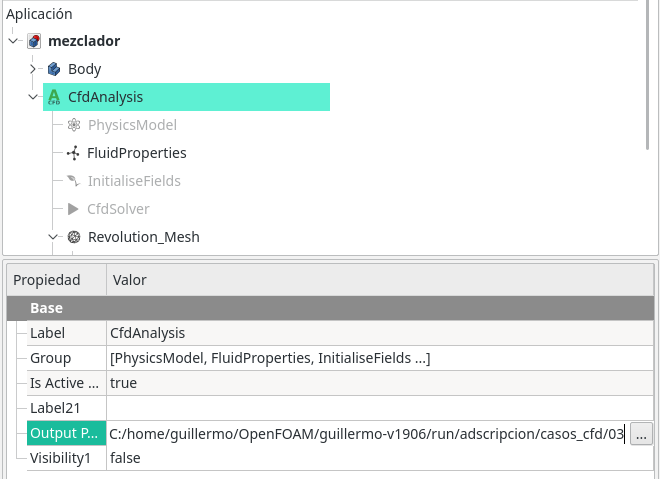
\includegraphics[width=0.7\textwidth]{Figuras/02_OUTPUTPATH.png}} \caption{Propiedad \textit{Output Path} en \textit{CfdAnalysis}} \label{fg:fc_outputpath}
\end{figure*}



Definimos las condiciones de contorno para cada cara de la geometría y ajustamos las propiedas del fluido y del solver. Ver las condiciones y propiedades correspondientes en los archivos del \href{https://github.com/guillerolle/casos_cfd/tree/master/03}{repositorio}. Una vez hecho esto tendremos un árbol similar a la de la figura \ref{fg:estructura_freecad}.

\begin{figure*}[htb]
	\centerline{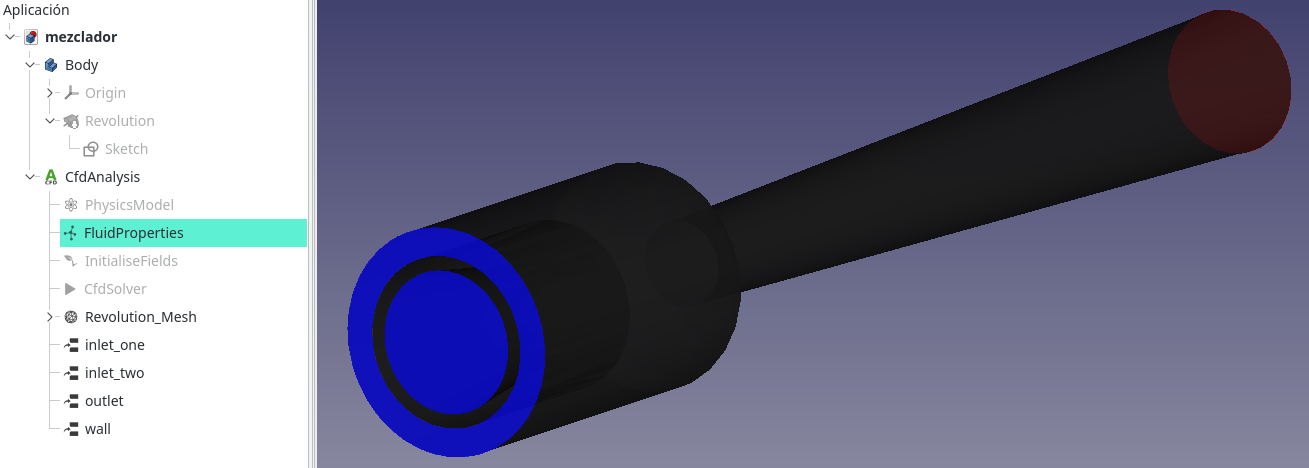
\includegraphics[width=0.7\textwidth]{Figuras/02_ESTRUCTURA_FREECAD.png}} \caption{Estructura básica del estudio CFD} \label{fg:estructura_freecad}
\end{figure*}

\subsection{Mallado}
Seleccionamos el sólido de revolución y elegimos la opción de crear una nueva malla a partir del sólido. Usamos el mallador \textbf{snappyHexMesh} en \textbf{3D} y un tamaño base de elemento 0.5mm. Usamos la utilidad para encontrar un punto dentro de la geometría y cerramos la ventana de tareas (todavía no ejecutar el caso de mallado). Vamos a crear además un refinamiento sobre las superficies de las paredes para tener una mejor definición de la capa límite. Para esto, seleccionar la malla (en el estudio CFD) y clickear en refinamiento de malla. Seleccionamos refinamiento por superficie y tamaño relativo de 0.5. Luego seleccionamos todas las superficies de pared.

Con esto estamos listo para escribir el caso de mallado y ejecutarlo. En la figura \ref{fg:pv_malla} se muestra la malla generada en el visualizador \textbf{ParaView}. Observar el refinamiento sobre las paredes. Tener en cuenta que \textbf{Paraview} presenta algunos errores en la visualización de la malla, pero el mallado es correcto. Comprobar ejecutando \texttt{checkMesh}. También corroborar que las regiones de entrada/salida estén definidas correctamente.

\begin{figure*}[htb]
	\centerline{
		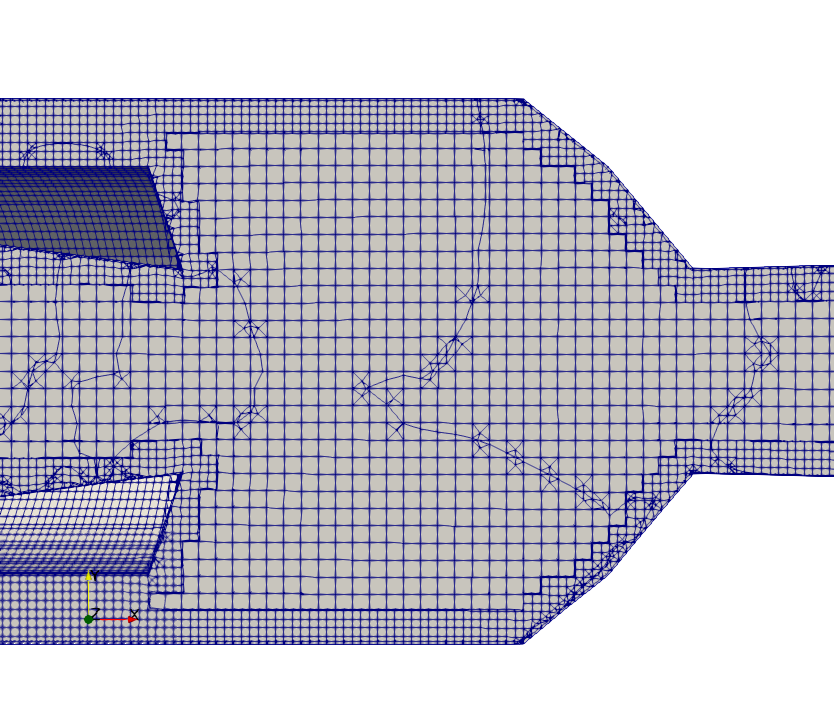
\includegraphics[width=0.4\textwidth]{Figuras/02_MALLA_CAMARA.png}
		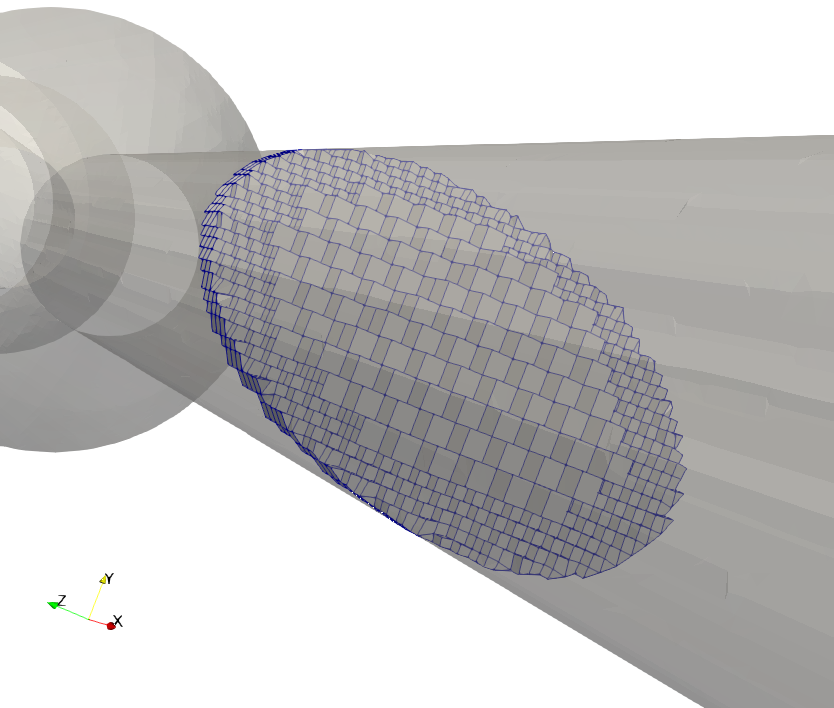
\includegraphics[width=0.4\textwidth]{Figuras/02_MALLA_SECCION.png}} \caption{Malla en cámara de mezcla (izquierda) y en sección interna del difusor de salida (derecha)} \label{fg:pv_malla}
\end{figure*}

\newpage
\section{SIMULACIÓN SIMPLEFOAM}
Una vez creada la malla y definidas las propiedas del solver (modelo estacionario, flujo incompresible, agua, etc.) abrimos la sección \textbf{CfdSolver} en \textbf{FreeCAD} y escribimos el caso. Antes de ejecutarlo, debemos realizar algunas modificaciones en los archivos \textit{fvSolution} y \textit{fvSchemes}. En el repositorio se encuentran los archivos \href{https://github.com/guillerolle/casos_cfd/tree/master/03/case/system/fvSolution.bkp}{fvSolution.bkp} y \href{https://github.com/guillerolle/casos_cfd/tree/master/03/case/system/fvSchemes.bkp}{fvSchemes.bkp}. Reemplazar los anteriores por éstos últimos para mejorar la convergencia de la simulación.

Se sugiere utilizar una utilidad como \href{https://meldmerge.org}{Meld} para comparar archivos y/o carpetas. En la figura \ref{fg:meld} se muestra esta utilidad comparando los archivos mencionados.

\begin{figure*}[htb]
	\centerline{
		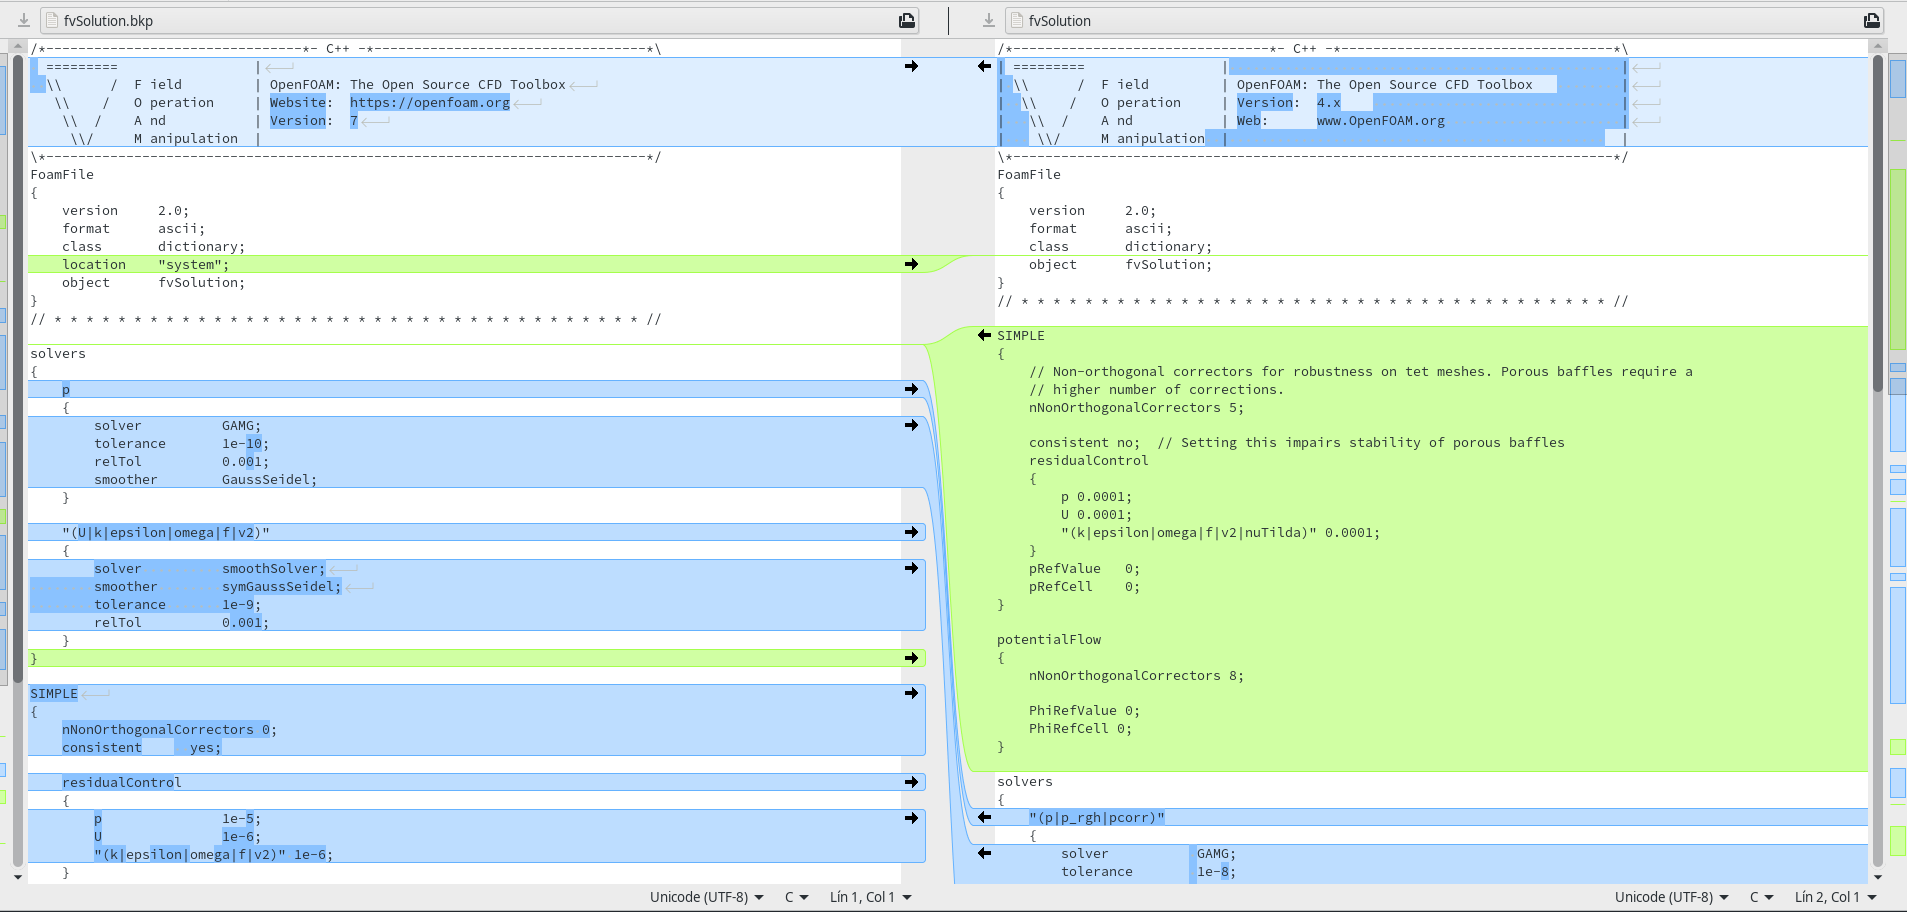
\includegraphics[width=0.8\textwidth]{Figuras/03_MELD.png}}
		 \caption{Comparación archivos fvSolution.bkp (izquierda) con fvSolution (derecha)} \label{fg:meld}
\end{figure*}

Volviendo a FreeCAD, podremos ejecutar la simulación con \textit{RUN}. Observar que la evolución de los residuales (figura \ref{fg:03_sf_residuales}) comienza a oscilar sobre un valor aproximadamente constante a partir de la iteración número 1000 sin llegar nunca a las tolerancias definidas en \textit{system/fvSolution}. 

\begin{figure*}[htb]
	\centerline{
		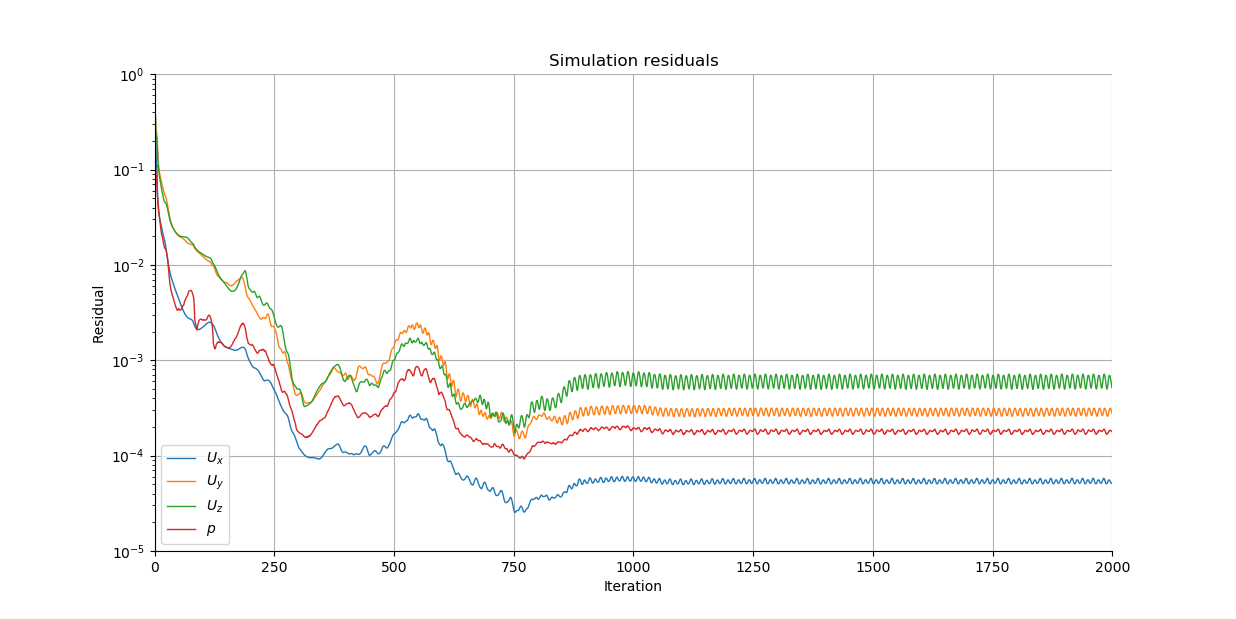
\includegraphics[width=0.8\textwidth]{Figuras/03_SF_RESIDUALES.png}}
	\caption{Evolución de residuales con simpleFoam} \label{fg:03_sf_residuales}
\end{figure*}

Sin necesidad de esperar a que termine de correr la simulación, podemos ver la evolución del perfil en ParaView. En la figura \ref{fg:03_sf_U} se muestra el campo de velocidades para una iteración bastante avanzada de la simulación (1700). Al comparar con pasos de tiempo consecutivos, no se aprecian grandes diferencias en los campos de velocidad o presión, por lo que asumiremos que la simulación fue satisfactoria.
FreeCAD descompone el caso en varios procesadores, por lo que para ver los resultados en ParaView debemos seleccionar "DecomposedCase".

\begin{figure*}[htb]
	\centerline{
		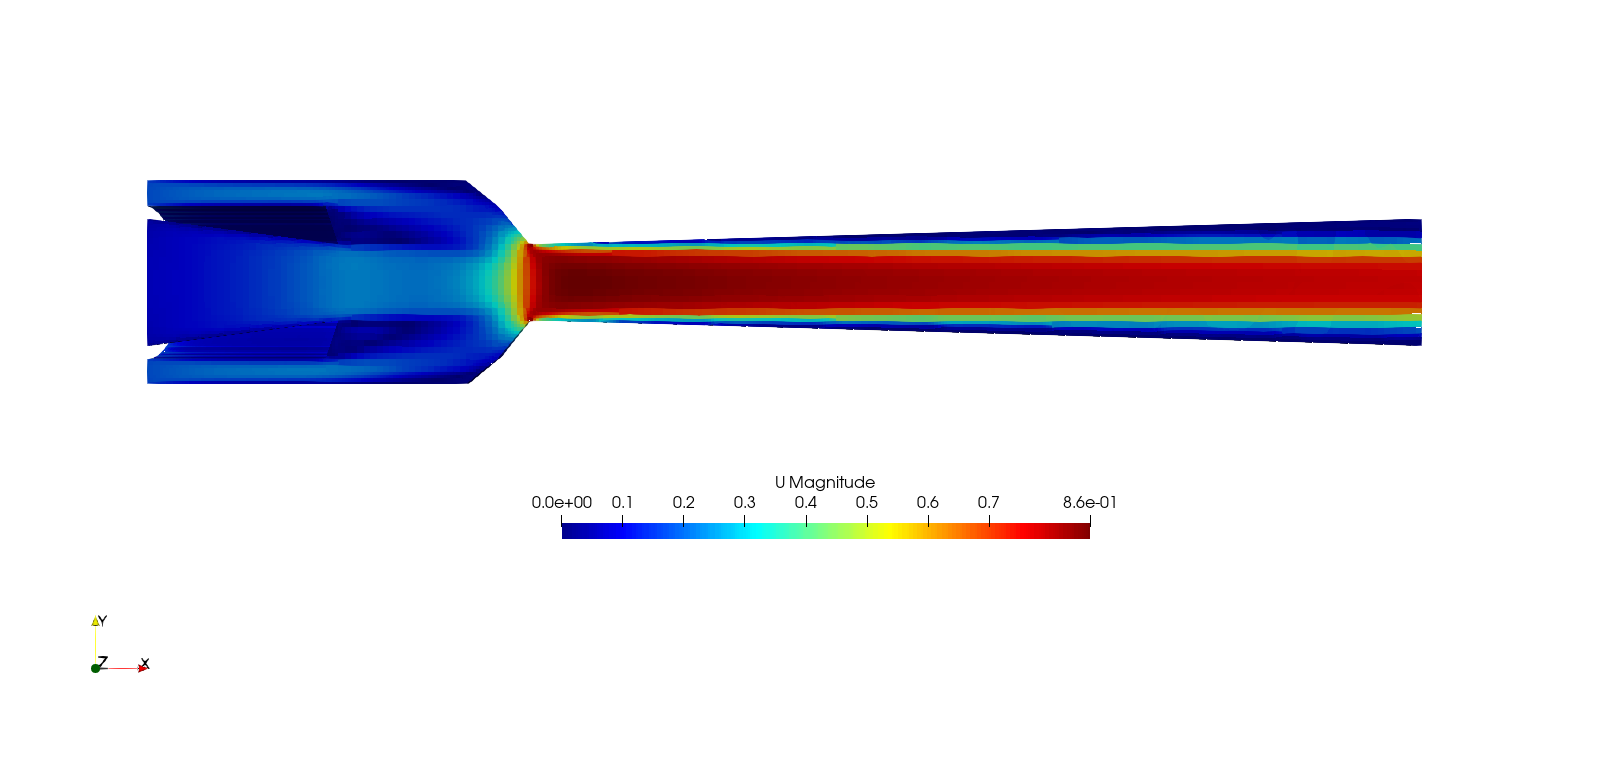
\includegraphics[width=0.8\textwidth]{Figuras/03_SF_U.png}}
	\caption{Campo de velocidad U obtenido} \label{fg:03_sf_U}
\end{figure*}

\subsection{Reconstrucción del caso}
Ya sabemos de los informes anteriores que necesitamos copiar el campo de presión y velocidad obtenidos con esta simulación en otro directorio que contenga el caso de la simulación RTD. Como el caso fue ejecutado en varios procesadores, en el directorio principal no encontraremos los pasos de simulación. Éstos se encuentran en las carpetas \texttt{processor*} y los archivos están divididos (caso descompuesto).

Para reconstruir el caso debemos ejecutar el comando \texttt{\$ reconstructPar} en el directorio \textit{case}. Ahora encontraremos los campos de presión y velocidad para la iteración 2000 en el directorio principal.

\section{SIMULACIÓN SCALARTRANSPORTFOAM}

Preparamos el caso de transporte escalar copiando la malla en \texttt{meshCase/constant/polyMesh} en el directorio \texttt{constant} del caso \texttt{RTD}. También traeremos de la simulación de \textit{simpleFoam} el campo de velocidad \texttt{2000/U} al directorio de condiciones iniciales \texttt{0/U} en \texttt{RTD}.
Ajustamos las condiciones en \texttt{system} según los valores del \href{https://github.com/guillerolle/casos_cfd/blob/master/03/RTD/system}{repositorio}

\subsection{Descomposición en varios procesadores}
En el diccionario \href{https://github.com/guillerolle/casos_cfd/blob/master/03/RTD/system/decomposeParDict}{system/decomposeParDict} se indica la cantidad de subprocesos que se usarán para correr la simulación. Ajustar este valor en función de la cpu dónde se ejecuta. En este caso, se utilizarán 4 procesadores.

Ejecutamos \texttt{\$ createPatch -overwrite} y luego \texttt{\$ decomposePar -force} en el directorio principal y aparecerán ahora directorios \texttt{processor*}. Ahora, con el siguiente comando podremos iniciar la simulación: \par 
\texttt{\$ mpirun -n 4 scalarTransportFoam -parallel | \\} 
\texttt{>  tee log.scalarTransportFoam}

En la figura \ref{fg:04_stf_res} se ven los residuales de esta simulación. Recordando que es una simulación en estado transitorio, se puede concluir que el solver llega a una solución constante a partir del 1er segundo de simulación aproximadamente.

\begin{figure*}[htb]
	\centerline{
		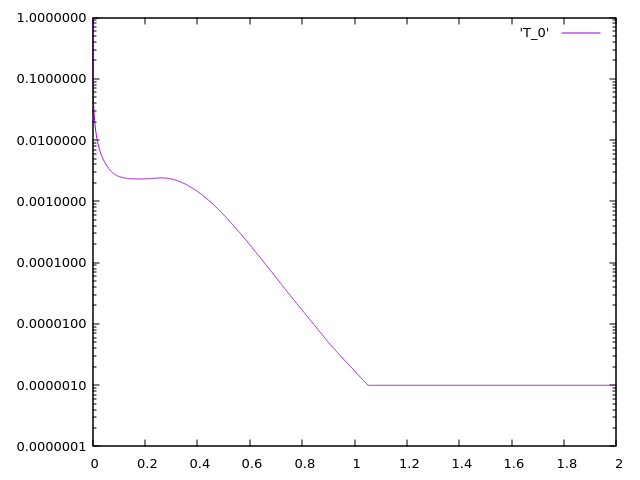
\includegraphics[width=0.8\textwidth]{Figuras/04_STF_RESIDUAL_T.png}}
	\caption{Evolución de residuales con simpleFoam} \label{fg:04_stf_res}
\end{figure*}

\section{POST-PROCESO}

Vamos a usar principalmente \textit{ParaView} para analizar los resultados. En la figura \ref{fg:05_stream_t} podemos ver unas líneas de traza coloreadas en función de la concentración de agroquímico. Se hizo la muestra sobre una línea paralela al eje 'Y' para facilitar la interpretación del campo tridimensional. Se observa que la mayor parte del mezclado se realiza, en realidad, justo después de la cámara de mezclado. Este fenómeno se puede adjudicar a que el flujo es laminar (por el modelo propuesto en la simulación), dificultando el mezclado dentro de la cámara.

\begin{figure*}[htb]
	\centerline{
		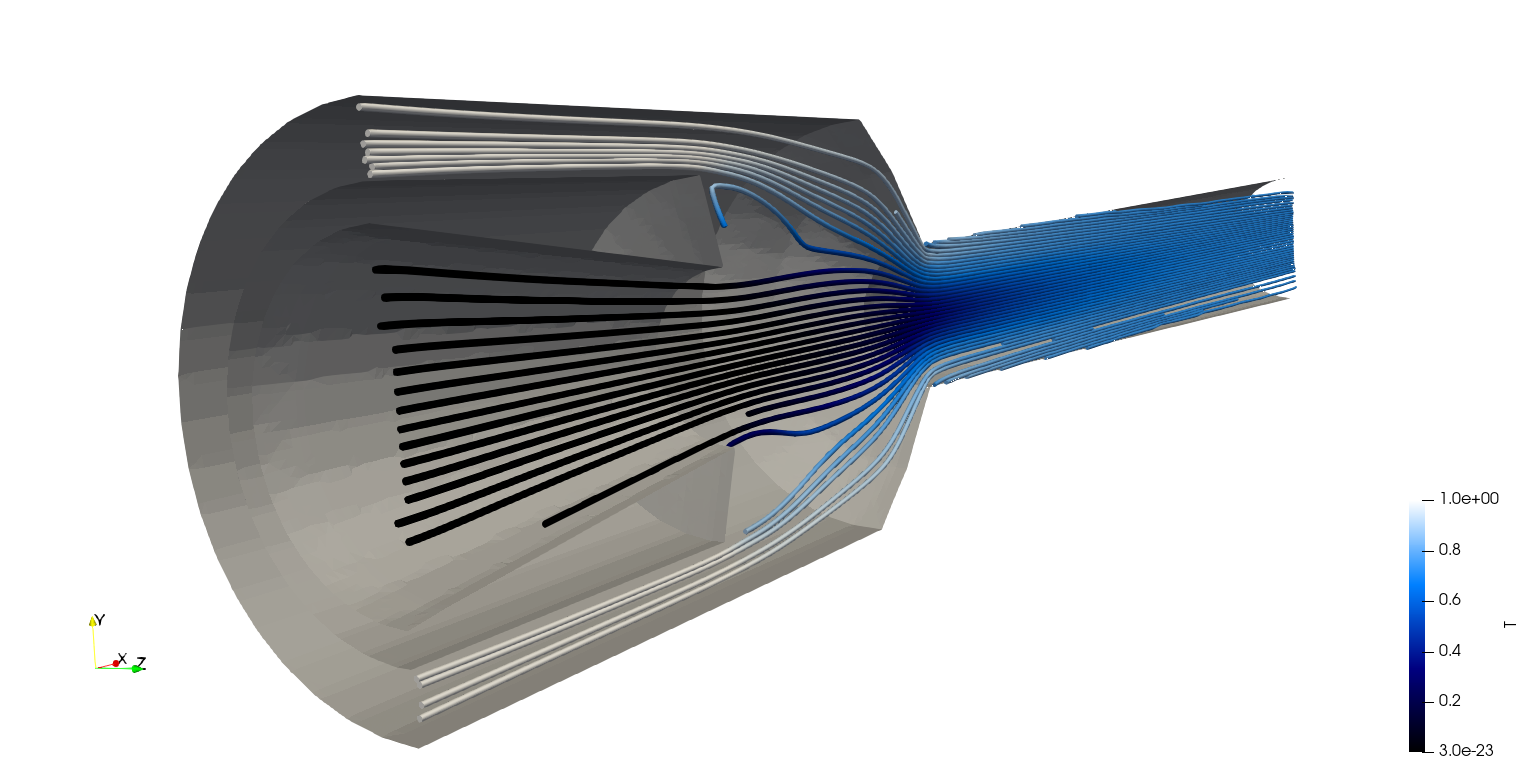
\includegraphics[width=0.8\textwidth]{Figuras/05_STREAMLINES_T.png}}
	\caption{Líneas de traza coloreadas según concentración de agroquímico} \label{fg:05_stream_t}
\end{figure*}

Con una rápida inspección visual parece ser que a la salida la concentración de agroquímico es aproximadamente 0.7. Usando la función de posproceso definida en el caso de OpenFOAM como \textit{patchAverage} calculamos la evolución de la concentración en la superficie de salida. El valor final es de 72\%. En la figura \ref{fg:05_avg_T} se muestra esta evolución.


\begin{figure*}[htb]
	\centerline{
		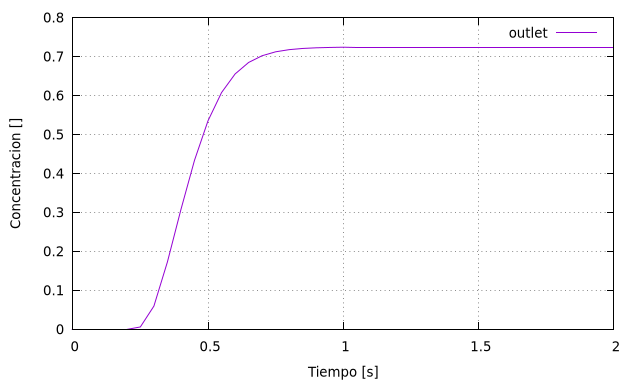
\includegraphics[width=0.6\textwidth]{Figuras/05_AVERAGE_T.png}
	}
	\caption{Evolución la concentración en la salida del dispositivo} \label{fg:05_avg_T}
\end{figure*}

Si hacemos varios cortes en distintas secciones del dispositivo podemos ver cómo varía la distribución de concentración en el eje 'X', como se muestra en la figura \ref{fg:05_STR_XY}. Observar que el agroquímico no llega a difundir perfectamente en la salida (color verde).


\begin{figure*}[htb]
	\centerline{
		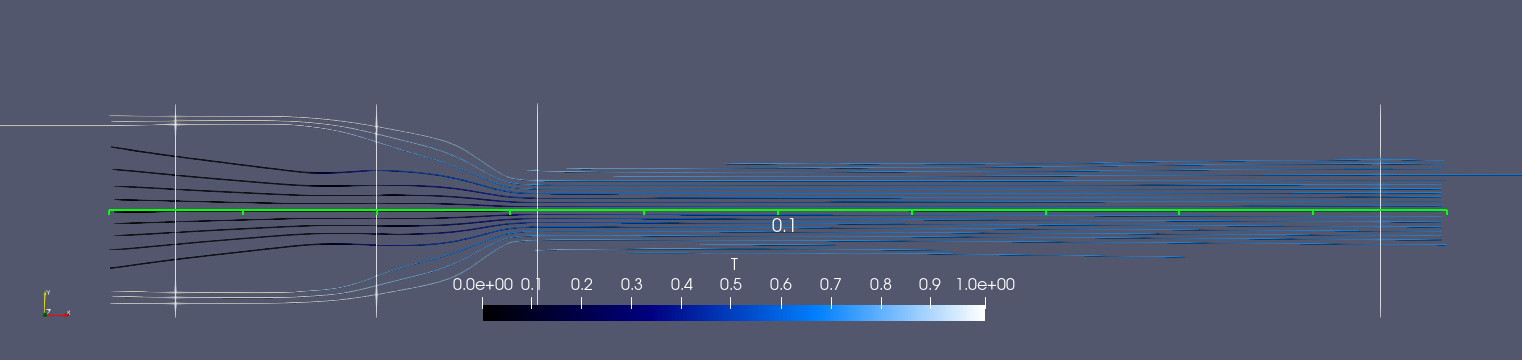
\includegraphics[width=0.8\textwidth]{Figuras/05_STREAM_DIVISIONES.png}
	}
	\centerline{
		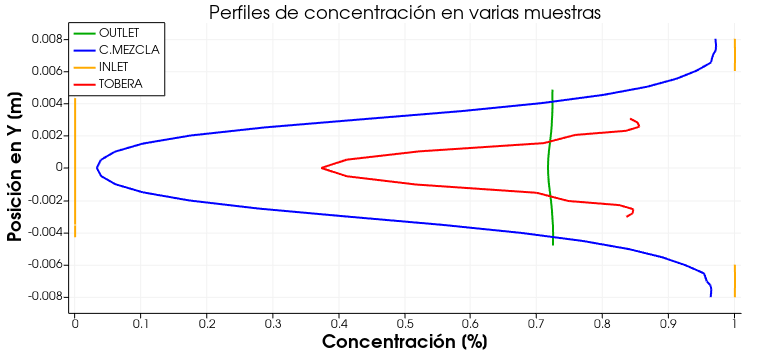
\includegraphics[width=0.8\textwidth]{Figuras/05_T_VARIAS.png}
	}
	\caption{Distribución de concentración de agroquímico en varias secciones del dispositivo} \label{fg:05_STR_XY}
\end{figure*}

Sería conveniente analizar más detalladamente la concentración en la superficie de salida del dispositivo. Si bien debería mantener una simetría respecto del eje del dispositivo, en la figura  \ref{fg:05_outlet} queda en evidencia que esto no sucede así. Una posible razón de este inconveniente, es la malla ortogonal alineada con los ejes cartesianos en todo el volumen de la muestra. 

\begin{figure*}[htb]
	\centerline{
		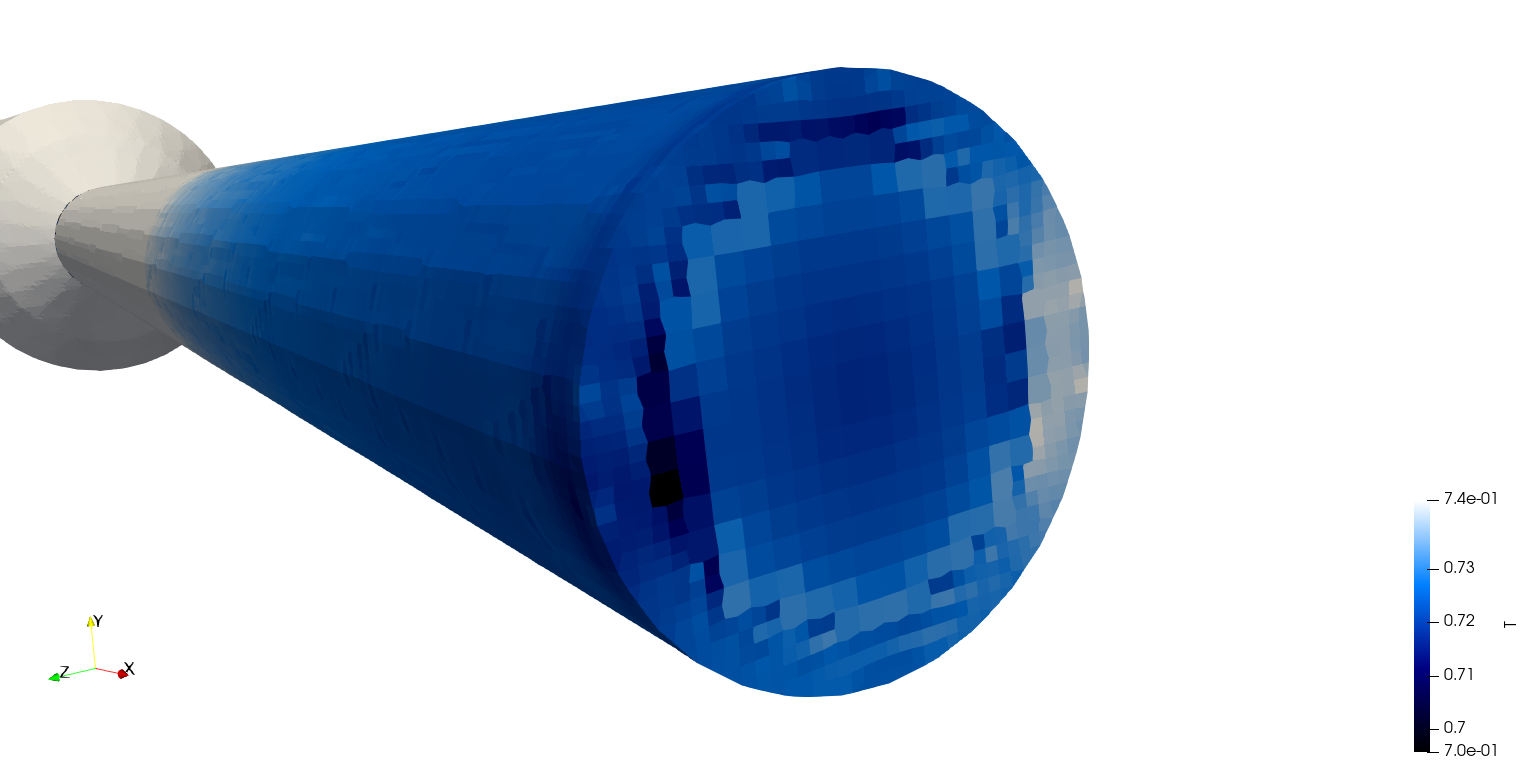
\includegraphics[width=0.8\textwidth]{Figuras/05_OUTLET_T.png}
	}
	\caption{Concentración en Outlet. Valores por celda} \label{fg:05_outlet}
\end{figure*}

Esto puede implicar errores en la interpolación entre celdas. Será diferente para celdas contenidas en el plano XY (que debería tener componentes de velocidad únicamente en X e Y) que una que esté girada a 45 grados respecto a un plano paralelo al YZ. En este caso, el método debería interpolar en dirección a vértices de las celdas hexahedrícas y no sobre caras o aristas, generando diferencias entre celdas de una misma sección. En la figura \ref{fg:05_hexa_glyph} se muestra esta idea.


\begin{figure*}[htb]
	\centerline{
		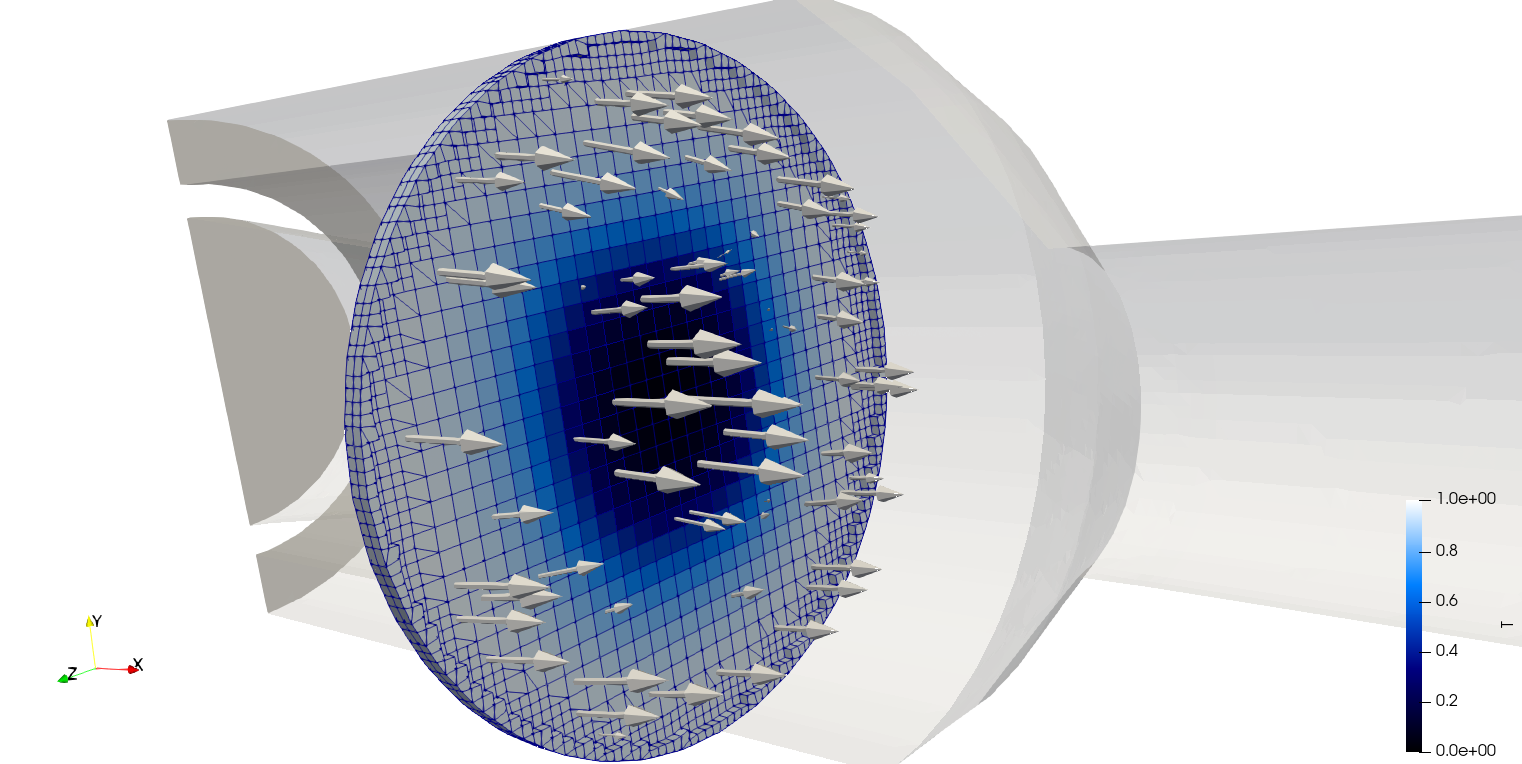
\includegraphics[width=0.8\textwidth]{Figuras/05_GLYPH_HEXA.png}
	}
	\caption{Malla ortogonal en un caso simétrico respecto a un eje} \label{fg:05_hexa_glyph}
\end{figure*}

Además, hay que tener en cuenta que el método no pudo reducir los residuales por más de $10^{-4}$, generando estas discrepancias con lo esperado. En ciertos casos, estas diferencias pueden ser perfectamente aceptables mientras que en otros no. Esto es criterio del ejecutante y de las exigencias que debe cumplir la simulación.

\section{CONCLUSIONES}
En este informe preparamos y ejecutamos el primer caso tridimensional del dispositivo. Generamos una malla sobre un modelo arbitrario creado en \textit{FreeCAD} y ejecutamos las simulaciones correspondientes. Surgieron dificultades con la convergencia de las simulaciones, mostrando de alguna manera la influencia del mallado sobre los resultados.

Además, se hace notar que los resultados esperados en cuanto a la concentración promedio en el outlet debería ser similar a los del \href{https://github.com/guillerolle/informes_cfd/blob/master/Informe02.pdf}{informe anterior} (34\%) pero en este caso dio valores muy diferentes (72\%). Revisando las condiciones impuestas, los valores de presión en los inlets debía ser de 300 kPa, pero por error se hicieron las simulaciones con 0.3 kPa. No se realiza la simulación nuevamente ya que éstos valores generan mayores inconvenientes en la convergencia (con los mismos diccionarios en \texttt{system} los residuales no bajan de $10^{-2}$) y se considera un trabajo innecesario para los fines prácticos de este informe y adscripción. Se prefiere continuar con una simulación más avanzada en el siguiente informe.

Aprovechando que las condiciones de la simulación no permiten resolver adecuadamente el caso en estado estacionario, el siguiente informe se va a realizar utilizando un solver transitorio \href{https://www.openfoam.com/documentation/guides/latest/doc/guide-applications-solvers-incompressible-pimpleFoam.html}{pimpleFoam}.

%\section*{AGRADECIMIENTOS} Los autores agradecen a ...
% ACKNOWLEDGEMENTS FOR FULL ARTICLES
%
%\bibliography{amcapaper}
\end{document}
